%%%%%%%%%%%%%%%%%%%%%%%%%%%%%%%%%%%%%%%%%%%%%%%%%%%%%%%%%%%%%%%%%%%%%%%%%%%%%%%%%%
% Template for FYP/ISP Report of NED University of Engg. & Tech., Karachi
% 2018 v1.0
% Created by Arsalan Khairani & Dr. Muhammad Ali Ismail
% https://github.com/ArsalanKhairani/report_latex_template
%%%%%%%%%%%%%%%%%%%%%%%%%%%%%%%%%%%%%%%%%%%%%%%%%%%%%%%%%%%%%%%%%%%%%%%%%%%%%%%%%%

% This template can be used as a to draft Final Year Project reports using LaTex.
% Created under the supervision of Dr. Muhammad Ali Ismail, Co-Chair CISD, NED, this
% provides a framework with all the necessary packages and formatting needed to provide a 
% quick start. That being said, it's also true that depending upon your needs, you
% might need to modify the template. Improvements to the templates are always welcomed,
% you can create a pull request to the Git repository mentioned above. I'll try to 
% comment the template as much as I can to explain the purpose of statements used and 
% how and what needs to be modified.

% Sidebar - Similar to programming, you can either create a very long single latex file with 
% all the imports and logic OR you can create multiple smaller modules. This template
% is constructed in modular format and thus this (the main file of the project) is very short.
% So let's get started!

% First step is to include all the packages (similar to programming). Like being said
% you could've done it in this file OR in some other file (like we did) and import it
% here. Check setup/preamble.tex for detailed description.
%%%%%%%%%%%%%%%%%%%%%%%%%%%%%%%%%%%%%%%%%%%%%%%%%%%%%%%%%%%%%%%%%%%%%%%%%%%%%%%%%%
% Template for FYP/ISP Report of NED University of Engg. & Tech., Karachi
% 2018 v1.0
% Created by Arsalan Khairani & Dr. Muhammad Ali Ismail
% https://github.com/ArsalanKhairani/report_latex_template
%%%%%%%%%%%%%%%%%%%%%%%%%%%%%%%%%%%%%%%%%%%%%%%%%%%%%%%%%%%%%%%%%%%%%%%%%%%%%%%%%%

% The first command is to define the document property.
\documentclass[12pt,a4paper,openright]{report}

%%%%%%%%%%%%%%%%%%%%%%%%%%%%%%%%%%%%%%%%%%%%%%%%
% Language, Encoding and Fonts.
% http://en.wikibooks.org/wiki/LaTeX/Internationalization
%%%%%%%%%%%%%%%%%%%%%%%%%%%%%%%%%%%%%%%%%%%%%%%%

% Select encoding of your inputs. Depends on
% your operating system and its default input
% encoding. Typically, you should use
%   Linux  : utf8 (most modern Linux distributions)
%            latin1 
%   Windows: ansinew
%            latin1 (works in most cases)
%   Mac    : applemac
% Notice that you can manually change the input
% encoding of your files by selecting "save as"
% an select the desired input encoding. 
\usepackage[utf8]{inputenc}

% Make latex understand and use the typographic
% rules of the language used in the document.
% csquotes is just a dependency package for babel.
\usepackage[english]{babel}
\usepackage{csquotes}

% Use the times new roman font
\usepackage{times}

%%%%%%%%%%%%%%%%%%%%%%%%%%%%%%%%%%%%%%%%%%%%%%%%
% Graphics and Tables
% http://en.wikibooks.org/wiki/LaTeX/Importing_Graphics
% http://en.wikibooks.org/wiki/LaTeX/Tables
% http://en.wikibooks.org/wiki/LaTeX/Colors
%%%%%%%%%%%%%%%%%%%%%%%%%%%%%%%%%%%%%%%%%%%%%%%%
% load a colour package
\usepackage{xcolor}
\definecolor{aaublue}{RGB}{33,26,82}% dark blue
% The standard graphics inclusion package
\usepackage{graphicx}
% Set up how figure and table captions are displayed
\usepackage{caption}
\captionsetup{%
  font=footnotesize,% set font size to footnotesize
  labelfont=bf % bold label (e.g., Figure 3.2) font
}
% Make the standard latex tables look so much better
\usepackage{array,booktabs}
% Enable the use of frames around, e.g., theorems
% The framed package is used in the example environment
\usepackage{framed}

%%%%%%%%%%%%%%%%%%%%%%%%%%%%%%%%%%%%%%%%%%%%%%%%
% Mathematics
% http://en.wikibooks.org/wiki/LaTeX/Mathematics
%%%%%%%%%%%%%%%%%%%%%%%%%%%%%%%%%%%%%%%%%%%%%%%%
% Defines new environments such as equation,
% align and split 
\usepackage{amsmath}
% Adds new math symbols
\usepackage{amssymb}
% Use theorems in your document
% The ntheorem package is also used for the example environment
% When using thmmarks, amsmath must be an option as well. Otherwise \eqref doesn't work anymore.
\usepackage[framed,amsmath,thmmarks]{ntheorem}
% Theorem & definition
\theoremstyle{plain}
\newtheorem{thm}{Theorem}[chapter] % reset theorem numbering for each chapter

\theoremstyle{plain}
\newtheorem{defn}[thm]{Definition} % definition numbers are dependent on theorem numbers
\newtheorem{exmp}[thm]{Example} % same for example numbers
% For floor function
\usepackage{mathtools}
\DeclarePairedDelimiter\ceil{\lceil}{\rceil}
\DeclarePairedDelimiter\floor{\lfloor}{\rfloor}

%%%%%%%%%%%%%%%%%%%%%%%%%%%%%%%%%%%%%%%%%%%%%%%%
% Page Layout
% http://en.wikibooks.org/wiki/LaTeX/Page_Layout
%%%%%%%%%%%%%%%%%%%%%%%%%%%%%%%%%%%%%%%%%%%%%%%%
\usepackage[left=3.0cm,right=3.0cm,top=3.0cm,bottom=2.5cm]{geometry}
% Modify how \chapter, \section, etc. look
% The titlesec package is very configureable
\usepackage{titlesec}
\titleformat{\chapter}[display]{\normalfont\large\bfseries}{\chaptertitlename\ \thechapter}{0.5cm}{\Large\centering}
\titlespacing*{\chapter}{0pt}{-50pt}{40pt}
\titleformat*{\section}{\normalfont\normalsize\bfseries}
\titleformat*{\subsection}{\normalfont\normalsize\bfseries}
\titleformat*{\subsubsection}{\normalfont\normalsize\bfseries}
\titleformat*{\paragraph}{\normalfont\normalsize\bfseries}

% Change the headers and footers
\usepackage{fancyhdr}
\fancyhf{} %delete everything
\renewcommand{\headrulewidth}{0pt} %remove the horizontal line in the header
\fancyhead[C]{- \thepage\ -} %page number on all pages
% Do not stretch the content of a page. Instead,
% insert white space at the bottom of the page
\raggedbottom
\setlength{\headheight}{15pt}

%%%%%%%%%%%%%%%%%%%%%%%%%%%%%%%%%%%%%%%%%%%%%%%%
% Bibliography
% http://en.wikibooks.org/wiki/LaTeX/Bibliography_Management
%%%%%%%%%%%%%%%%%%%%%%%%%%%%%%%%%%%%%%%%%%%%%%%%
\usepackage[sorting=none]{biblatex}
\addbibresource{bib/mybib.bib}

%%%%%%%%%%%%%%%%%%%%%%%%%%%%%%%%%%%%%%%%%%%%%%%%
% Misc
%%%%%%%%%%%%%%%%%%%%%%%%%%%%%%%%%%%%%%%%%%%%%%%%
% Add bibliography and index to the table of
% contents
\usepackage[nottoc]{tocbibind}
% Add the command \pageref{LastPage} which refers to the
% page number of the last page
\usepackage{lastpage}
% Add todo notes in the margin of the document
\usepackage[
%  disable, %turn off todonotes
  colorinlistoftodos, %enable a coloured square in the list of todos
  textwidth=\marginparwidth, %set the width of the todonotes
  textsize=scriptsize, %size of the text in the todonotes
  ]{todonotes}

% ability to merge multiple rows in table
\usepackage{multirow}

% it creates a tab indentation before paragraph.
\setlength{\parindent}{2em}

% By default, tab indentation isn't enabled for 1st para of chapter,
% this package will enable it for 1st paragraph.
\usepackage{indentfirst}

% package with shortcuts for single and double line spacing
\usepackage{setspace}

% Though on the master.tex, we've mentioned that \pagestyle
% command would reset the page style, but unfortunately, it
% doesn't word for pages with chapters. The below is a hack
% to make chapter follow the empty style.
\patchcmd{\chapter}{plain}{empty}{}{}

%%%%%%%%%%%%%%%%%%%%%%%%%%%%%%%%%%%%%%%%%%%%%%%%
% Hyperlinks
% http://en.wikibooks.org/wiki/LaTeX/Hyperlinks
%%%%%%%%%%%%%%%%%%%%%%%%%%%%%%%%%%%%%%%%%%%%%%%%
% Enable hyperlinks and insert info into the pdf
% file. Hypperref should be loaded as one of the 
% last packages
\usepackage{hyperref}
\hypersetup{%
	plainpages=false,%
	pdfauthor={Author(s)},%
	pdftitle={Title},%
	pdfsubject={Subject},%
	bookmarksnumbered=true,%
	colorlinks=false,%
	citecolor=black,%
	filecolor=black,%
	linkcolor=black,% you should probably change this to black before printing
	urlcolor=black,%
	pdfstartview=FitH%
}

%%%%%%%%%%%%%%%%%%%%%%%%%%%%%%%%%%%%%%%%%%%%%%%%
% Algorithms
% https://en.wikibooks.org/wiki/LaTeX/Algorithms
%%%%%%%%%%%%%%%%%%%%%%%%%%%%%%%%%%%%%%%%%%%%%%%%
\usepackage[ruled,vlined]{algorithm2e}

%%%%%%%%%%%%%%%%%%%%%%%%%%%%%%%%%%%%%%%%%%%%%%%%
% Plots
% https://en.wikibooks.org/wiki/LaTeX/PGF/TikZ
%%%%%%%%%%%%%%%%%%%%%%%%%%%%%%%%%%%%%%%%%%%%%%%%
\usepackage{pgfplots}
\pgfplotsset{compat=1.14}
\usepgfplotslibrary{groupplots}
\usetikzlibrary{matrix}

%%%%%%%%%%%%%%%%%%%%%%%%%%%%%%%%%%%%%%%%%%%%%%%%
% Code
% https://en.wikibooks.org/wiki/LaTeX/Source_Code_Listings
%%%%%%%%%%%%%%%%%%%%%%%%%%%%%%%%%%%%%%%%%%%%%%%%
\usepackage{listings}
\lstset{
  columns=fullflexible,
  frame=single,
  breaklines=true,
  postbreak=\mbox{\textcolor{red}{$\hookrightarrow$}\space},
}


% The latex document always starts with a begin{document} command and ends with end{document} command.
\begin{document}

  % front_page.tex is the cover page of hard binded book. It's according to the format
  % specified by NEDUET. However, to get it printed on a hard cover consult the binder.
  \begin{titlepage}
  \centering
  {\Large\textbf{Project Title}}
  
  \vspace{4cm}
  {\large\textbf{B.E (CIS) PROJECT REPORT\\ by\\ \vspace{0.5cm} Name of Group Leader}}

  \vspace{2cm}
  \begin{figure}[ht]
    \centering
    
\includegraphics[width=6cm]{images/ned_logo.png}
  \end{figure}
  
  \vfill
  \textbf{Department of Computer and Information Systems Engineering}
  \vspace{1cm}

  \textbf{NED University of Engg. \& Tech.,\\
  Karachi-75270}
\end{titlepage}
\clearpage
  
  % first_page.tex is the internal cover page.
  % This is the cover page of the report. Note the titlepage environment would
% make sure that formatting defined for content isn't used in current page. Needless
% to say, title page is single page only.
\begin{titlepage}

  % Everything on the title page needs to be center aligned.
  \centering
  
  % Add your Project title here.
  {\Large\textbf{Project Title}}
  
  % Add some space using vspace
  \vspace{2cm}
  {\large\textbf{B.E (CIS) PROJECT REPORT}}
  \vspace{2cm}
  
  % Next, group members names and roll numbers
  \textbf{Project Group:}
  \begin{table}[ht]
    \centering
    \begin{tabular}{l l}
      NAME OF MEMBER 1 & CS-01 \\
      NAME OF MEMBER 2 & CS-02 \\
      NAME OF MEMBER 3 & CS-03 \\
      NAME OF MEMBER 4 & CS-04 \\
    \end{tabular}
  \end{table}
 
  \textbf{Batch:} 2011-12
  \vspace{2cm}

  {\large\textbf{Project Advisor(s):}\\
  Name of Advisor (Internal Advisor)\\
  Name of Advisor (External Advisor (if any))}
  \vspace{1cm}

  \textbf{May} 2018
  
  \vfill
  \textbf{Department of Computer and Information Systems Engineering}
  \vspace{1cm}

  \textbf{NED University of Engg. \& Tech.,\\Karachi-75270}
\end{titlepage}

  
  % The next section contains things like abstract, acknowledgements, table of contents
  % etc. Note the use of pagestyle command, this command resets the header and footer
  % style so that the following pages doesn't get the header & footer like the main
  % content. In other words, we don't want page numbers on the following pages.
  % However, following the pagestyle statement, you'd see that we've used pagenumbering
  % command, this commands sets the format of page numbers. We need it here otherwise,
  % the following pages would get page numbers as well and though pagestyle can
  % make them disappear, we'd see those page numbers in table of contents.
  % Finally, the cleardoublepage command is to end the current page. Removing this
  % command could result in improper page numbering.
  \doublespacing
  \pagestyle{empty}
  \pagenumbering{roman}
  \chapter*{Abstract}\label{ch:abstract}
\textit{The abstract of the report will be just after the Internal Title Page. The abstract should be brief and should be about half a page but certainly not more than one page. 12-point Italic Times New Roman Font is used.}

  \chapter*{Acknowledgments}\label{ch:acknowledgments}
The acknowledgement page (if any).

  \tableofcontents
  \listoffigures
  \listoftables
  \cleardoublepage
  
  % Here is the main content of the report. Note that we're now using fancy pagestyle
  % and also using the arabic numerals for page numbers.
  \pagestyle{fancy}
  \pagenumbering{arabic}
  \chapter{Introduction}\label{ch:introduction}
The first chapter of the report should be the introduction chapter. The format shown on the first page of this first chapter must be followed in all chapters. The text is double-line spaced. 

Every new paragraph starts with an indentation of one tab space. The font is Regular 12-point Times New Roman and fully justified. The sections are numbered according to the number of Chapter.

\section{Figures and Tables}
There can be several sections within every chapter. The start of every section is indented (similar to paragraph). The number of sections depends upon the text. The sections are numbered according to the chapter number. For example for chapter 1, the sections are 1.1, 1.2, 1.3 and so on. 

The figures and tables are also numbered according to chapter number and will be displayed as same on the list of figures and list of tables, if applicable. You can add an image as shown below and reference it as figure \ref{fig:sample_image}. To reference a figure caption and label are necessary \textbf{and in the same order}. You can read more about inserting images at: \url{https://www.sharelatex.com/learn/Inserting_Images}.

\begin{figure}[ht]
  \centering
  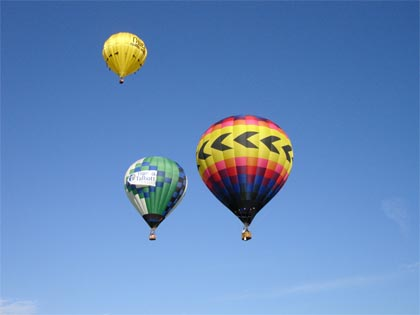
\includegraphics[width=6cm]{images/sample_image.jpeg}
  \caption{Sample Image}
  \label{fig:sample_image}
\end{figure}

A sample table is show below, you can reference it as \ref{tab:sample_table}. Note that the prefix "fig:" in case of figure and "tab:" in case of table isn't required but it's considered as good practice. You can read more about tables at: \url{https://www.sharelatex.com/learn/Tables}.

\begin{table}[ht]
  \centering
  \caption{Sample Table}
  \label{tab:sample_table}
  \begin{tabular}{ |c|c|c|c| } 
    \hline
    col1 & col2 & col3 \\
    \hline
    \multirow{3}{4em}{Multiple row} & cell2 & cell3 \\ 
    & cell5 & cell6 \\ 
    & cell8 & cell9 \\ 
    \hline
  \end{tabular}
\end{table}

\section{References}
You can add a citation in the text using the cite command as \cite{big} or multiple as \cite{big,small}. Citing a paper or journal would automatically add it's details in References section.

\subsection{Subsection within a section}
There can be subsections within the sections. The format of the subsections should be the same as shown in this example. The subsections should also be numbered according to the number of chapter. For example for chapter 1, section 1.1, subsections should be numbered as 1.1.1, 1.1.2 and so on.

  \chapter{Name of Chapter 2}\label{ch:chapter_2}
This is the chapter number 2 of the report.

\section{Plots}
You can construct plots with latex as well using pgfplots package. Read \url{https://www.sharelatex.com/learn/Pgfplots_package} for more details. Below is a sample plot.

\begin{figure}[ht]
  \centering
  \begin{tikzpicture}
    \begin{axis}
      \addplot[color=red]{exp(x)};
    \end{axis}
  \end{tikzpicture}
\end{figure}

\section{How to}
To use LaTex you can either install it (and it's packages) on the system. Ton of resources on Internet with instructions. Or you can use online tools to do that.
\begin{itemize}
\item \url{https://www.overleaf.com/}
\item \url{https://www.sharelatex.com/}
\end{itemize}

  
  % The final section of our report is bibliography. You can add you references in
  % bib/mybib.bib and they would automatically appear here, if cited.
  % The linespread{1} command is changing the linespacing to single space unlike the
  % rest of the document which is double spaced.
  \linespread{1}
  \printbibliography[heading=bibintoc,title={References}]
  \label{bib:mybiblio}
  
% And that's al1.
\end{document}
